\documentclass[11pt]{report}

% Paquetes y configuraciones adicionales
\usepackage{amsmath, amsthm, amssymb} % Paquetes matemáticos
\usepackage[utf8]{inputenc} % Codificación .tex
\usepackage{graphicx}
\usepackage[export]{adjustbox}
\usepackage{caption}
\usepackage{float}
\usepackage{titlesec}
\usepackage{geometry}
\usepackage[hidelinks]{hyperref}
\usepackage{titling}
\usepackage{titlesec}
\usepackage{parskip}
\usepackage{wasysym}
\usepackage{tikzsymbols}
\usepackage{fancyvrb}
\usepackage{xurl}
\usepackage{hyperref}
\usepackage{subcaption}
\usepackage{tikz}
\usepackage{listings}
\usepackage{xcolor}

\usepackage[spanish]{babel}

\newcommand{\subtitle}[1]{
  \posttitle{
    \par\end{center}
    \begin{center}\large#1\end{center}
    \vskip0.5em}
}

% Configura los márgenes
\geometry{
  left=2cm,   % Ajusta este valor al margen izquierdo deseado
  right=2cm,  % Ajusta este valor al margen derecho deseado
  top=3cm,
  bottom=3cm,
}

% Configuración de los títulos de las secciones
\titlespacing{\section}{0pt}{\parskip}{\parskip}
\titlespacing{\subsection}{0pt}{\parskip}{\parskip}
\titlespacing{\subsubsection}{0pt}{\parskip}{\parskip}

% Redefinir el formato de los capítulos y añadir un punto después del número
\makeatletter
\renewcommand{\@makechapterhead}[1]{%
  \vspace*{0\p@} % Ajusta este valor para el espaciado deseado antes del título del capítulo
  {\parindent \z@ \raggedright \normalfont
    \ifnum \c@secnumdepth >\m@ne
        \huge\bfseries \thechapter.\ % Añade un punto después del número
    \fi
    \interlinepenalty\@M
    #1\par\nobreak
    \vspace{10pt} % Ajusta este valor para el espacio deseado después del título del capítulo
  }}
\makeatother

% Configura para que cada \chapter no comience en una pagina nueva
\makeatletter
\renewcommand\chapter{\@startsection{chapter}{0}{\z@}%
    {-3.5ex \@plus -1ex \@minus -.2ex}%
    {2.3ex \@plus.2ex}%
    {\normalfont\Large\bfseries}}
\makeatother

% Configurar los colores para el código
\definecolor{codegreen}{rgb}{0,0.6,0}
\definecolor{codegray}{rgb}{0.5,0.5,0.5}
\definecolor{codepurple}{rgb}{0.58,0,0.82}
\definecolor{backcolour}{rgb}{0.95,0.95,0.92}

% Configurar el estilo para el código
\lstdefinestyle{mystyle}{
  backgroundcolor=\color{backcolour},   
  commentstyle=\color{codegreen},
  keywordstyle=\color{magenta},
  numberstyle=\tiny\color{codegray},
  stringstyle=\color{codepurple},
  basicstyle=\ttfamily\footnotesize,
  breakatwhitespace=false,         
  breaklines=true,                 
  captionpos=b,                    
  keepspaces=true,                 
  numbers=left,                    
  numbersep=5pt,                  
  showspaces=false,                
  showstringspaces=false,
  showtabs=false,                  
  tabsize=2
}

% Configurar el estilo para el código en C++ y CUDA con colores
\lstset{
  style=mystyle,
  language=C++,
  morekeywords={__global__, __device__, __host__},
  deletekeywords={__global__, __device__, __host__}
}

%==============================================================================
% Cosas para la documentación LateX
% % Sangría
% \setlength{\parindent}{1em}Texto

% % Quitar sangría
% \noindent

% % Punto
% \CIRCLE \ \ \textbf{Texto} \emph{algo}
% \begin{itemize}
%   \item \textbf{Negrita:} Texto
%   \item \textbf{Negrita:} Texto
% \end{itemize}

% % Introducir código
% \begin{center}
%   \begin{BVerbatim}
%     ... Código
%   \end{BVerbatim}
% \end{center}

% Poner una imagen
% \begin{figure}[H]
%   \centering
%   \includegraphics[scale=0.55]{img/}
%   \caption{Exportación de la base de datos en formato sql}
%   \label{fig:exportación de la base de datos en formato sql}
% \end{figure}

% Poner dos imágenes
% \begin{figure}[H]
%   \begin{subfigure}{0.5\textwidth}
%     \centering
%     \includegraphics[scale=0.45]{img/}
%     \caption{Texto imagen 1}
%   \end{subfigure}%
%   \begin{subfigure}{0.5\textwidth}
%     \centering
%     \includegraphics[scale=0.45]{img/}
%     \caption{Texto imagen 2}
%   \end{subfigure}
%   \caption{Texto general}
% \end{figure}

% % Poner una tabla
% \begin{table}[H]
%   \centering
%   \begin{tabular}{|c|c|c|c|}
%     \hline
%     \textbf{Campo 1} & \textbf{Campo 2} & \textbf{Campo 3} & \textbf{Campo 4} \\ \hline
%     Texto & Texto & Texto & Texto \\ \hline
%     Texto & Texto & Texto & Texto \\ \hline
%     Texto & Texto & Texto & Texto \\ \hline
%     Texto & Texto & Texto & Texto \\ \hline
%   \end{tabular}
%   \caption{Nombre de la tabla}
%   \label{tab:nombre de la tabla}
% \end{table}

% % Poner codigo de un lenguaje a partir de un archivo
% \lstset{style=mystyle}
% The next code will be directly imported from a file
% \lstinputlisting[language=Python]{code.py}

% “Texto entre comillas dobles”

%==============================================================================

\begin{document}

% Portada del informe
\title{Filtro FIR}
\subtitle{Arquitecturas Avanzadas y de Propósito Específico}
\author{Cheuk Kelly Ng Pante (alu0101364544@ull.edu.es)}
\date{\today}

\maketitle

\pagestyle{empty} % Desactiva la numeración de página para el índice

% Índice
\tableofcontents

% Nueva página
\cleardoublepage

\pagestyle{plain} % Vuelve a activar la numeración de página
\setcounter{page}{1} % Reinicia el contador de página a 1

% Secciones del informe
% Capitulo 1
\chapter{Introducción}
FIR es un acrónimo en inglés para \emph{Finite Impulse Response} o Respuesta Finita al Impulso.
Se trata de un tipo de filtro digital que si su entrada es un impulso (una delta de Kronecker), su salida 
es un número limitado de términos no nulos. Este tipo de filtro se utiliza comúnmente en aplicaciones
de procesamiento de señales, como en la industria de las telecomunicaciones, el procesamiento de audio
y la ingeniería de control.

Su expresión en el dominio $n$ es la siguiente:
\begin{equation*}
  y_n = \sum_{k=0}^{N-1} b_k x_{n-k}
\end{equation*}

donde $x_n$ es la entrada, $y_n$ es la salida, $b_k$ son los coeficientes del filtro y $N$ es el orden del filtro.

La estructura básica de un filtro FIR es la siguiente:
\begin{figure}[H]
  \centering
  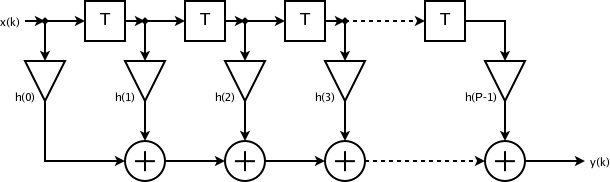
\includegraphics[scale=0.45]{img/FIR_estr.png}
  \caption{Estructura básica de un filtro FIR}
  \label{fig:estructura básica de un filtro fir}
\end{figure}

% Capitulo 2
\chapter{Características del proyecto}
El proyecto se divide en 5 versiones de filtros FIR:
\begin{itemize}
  \item Versión 0: Filtro FIR base
  \item Versión 1: Filtro FIR mejorado
  \item Versión 2: Incluye el uso de keywords, como \textbf{const} y \textbf{restrict}
  \item Versión 3: Desenrrollado manual y optimizacion de bucles, condicionales, etc.
  \item Versión 4: Utilización de \textbf{pragmas}
  \item Versión 5: Uso de \textbf{intrínsecos}
\end{itemize}

En cada versión incluye la implementación de un filtro FIR, dependiendo de la versión, y la lectura de los valores
de los coeficientes (Coeficientes.csv) y los valores de los datos de entrada (musica4.csv).

En cuanto al profiling se optado por usar \emph{clock()}, que es una función que mide el tiempo de ejecución de un programa. En principio
se pensó en usar \emph{gprof}, que es una herramienta de análisis de rendimiento para aplicaciones UNIX, pero no se pudo ya que los tiempos
de ejecución eran muy pequeños y no se podía medir correctamente.

Además, se ha calculado los ciclos de reloj de cada versión del filtro FIR. Para ello, se ha creado una función utilizando la instrucción
\emph{rdtsc} (Real Time Stamp Counter) que mide el número de ciclos de reloj desde el último reinicio. La función es la siguiente:
\begin{lstlisting}
uint64_t rdtsc(){
  unsigned int lo, hi;
  __asm__ __volatile__("rdtsc" : "=a"(lo), "=d"(hi));
  return ((uint64_t)hi << 32) | lo;
}
\end{lstlisting}

Lo que hace la función es utiliza la instrucción de ensamblador \emph{rdtsc} para leer el contador de tiempo de la CPU, y devuelve este 
valor como un número de 64 bits pero dividido en dos partes de 32 bits, \emph{lo} es la parte baja y \emph{hi} es la parte alta. Entonces,
se ejecuta la instrucción \emph{\_\_asm\_\_ \_\_volatile\_\_} que es una instrucción de ensamblador en línea que se utiliza para incrustar código
ensamblador en el código C.

El \emph{profiling} se ha hecho de la siguiente forma:
\begin{lstlisting}
start_cycle = rdtsc();
start = clock();
// --- Codigo a medir ---
end = clock();
end_cycle = rdtsc();
\end{lstlisting}

Por otra parte, para calcular el tiempo de ejecución y los ciclos de reloj se ha repetido \emph{N} veces, para obtener un promedio de los valores.
En este caso, se ha decidido hacer 1000 repeticiones, pero se puede cambiar el valor de \emph{N}
ya que se define como una constante en cada versión del filtro FIR.
\begin{lstlisting}
#define REPETICIONES 1000

// Aplicacion del filtro FIR
for (i = 0; i < REPETICIONES; i++) {
  start_cycle = rdtsc();
  start = clock();
  firfilter(vector_coef, vector_in, result);
  end = clock();
  end_cycle = rdtsc();

  elapsed = (double)(end - start) * 1000.0 / CLOCKS_PER_SEC;
  mean_time[i] = elapsed;
  mean_cycles[i] = end_cycle - start_cycle;
}
\end{lstlisting}

\newpage

% Capitulo 3
\chapter{Implementaciones}
\section*{Lectura de los coeficientes}
Para leer los coeficientes del filtro FIR se ha creado la siguiente función:
\begin{lstlisting}
float* inicializacion_coeficientes() {
  float* vector_coeficientes = (float*)malloc(COEF * sizeof(float));
  int i = 0;
  FILE* fich_coef = fopen("../data/Coeficientes.csv", "r");
  if (fich_coef == NULL) {
    printf("Error al abrir el archivo\n");
    exit(1);
  }

  while (fscanf(fich_coef, "%f", &vector_coeficientes[i]) != EOF && i < COEF) {
    i++;
  }
  fclose(fich_coef);

  return vector_coeficientes;
}
\end{lstlisting}

Lo que se hace es abrir el archivo \emph{Coeficientes.csv} que contiene los valores de los coeficientes del filtro FIR, y se lee cada valor
hasta que se llegue al final del archivo o se haya leído todos los valores. Luego, se cierra el archivo y se devuelve el vector de coeficientes.

\section*{Lectura de los datos de entrada}
Para leer los datos de entrada del filtro FIR se ha creado la siguiente función:
\begin{lstlisting}
float* inicializacion_vector_in() {
  float* array_data = (float*)malloc(N * sizeof(float));

  int i = 0;
  FILE* file_data = fopen("../data/musica4.csv", "r");
  if (file_data == NULL) {
    printf("Error al abrir el archivo\n");
    exit(1);
  }

  while (fscanf(file_data, "%f", &array_data[i]) != EOF && i < N) {
    i++;
  }

  fclose(file_data);

  return array_data;
}
\end{lstlisting}

Para la lectura de los datos de entrada se hace lo mismo que en la lectura de los coeficientes, se abre el archivo \emph{musica4.csv} que contiene
los valores de los datos de entrada, se leen los valores hasta que se llegue al final del archivo o se haya leído todos los valores y se cierra el archivo.

\newpage

\section{Versión base}
Para la implementación base se ha hecho la función \emph{firfilter()} que recibe los coeficientes del filtro FIR y los datos de entrada como punteros a float,
y devuelve un puntero a float con los valores de la salida del filtro FIR. La función es la siguiente:

\begin{lstlisting}
float* firfilter(float* vector_coef, float* vector_data) {
  float* result = (float*)malloc((N + COEF - 1) * sizeof(float));
  int i, j;
  for (i = 0; i < N + COEF - 1; i++) {
    result[i] = 0;
    for (j = 0; j < COEF; j++) {
      if (i - j >= 0 && i - j < N) {
        result[i] += vector_coef[j] * vector_data[i - j];
      }
    }
  }

  return result;
}
\end{lstlisting}

Lo que hace la función es inicializar un vector de float con el tamaño de la suma de los tamaños de los vectores de coeficientes y de los datos de entrada.
Luego, se inicializa un bucle que recorre el vector de salida, y dentro de este bucle se inicializa otro bucle que recorre el vector de coeficientes.
Dentro de este segundo bucle se comprueba si el índice de la salida menos el índice del bucle interno es mayor o igual a 0 y menor que el tamaño del vector de datos de entrada.
Si se cumple la condición, se multiplica el valor del coeficiente por el valor del dato de entrada y se suma al valor de la salida.

\section{Versión 1}
Para la versión 1 se ha mejorado la implementación base del filtro FIR. Lo que se ha hecho es trabajar directamente con los punteros de los vectores de coeficientes,
de los datos de entrada y de la salida. Usar punteros directamente y no devolver un puntero a float con los valores de la salida del filtro FIR es más eficiente. Además, 
se ha eliminado la condición del bucle interno, ya que se ha comprobado que no es necesario.

\begin{lstlisting}
void firfilter(float* vector_coef, float* vector_data, float* result) {
  int i, j;
  for (i = 0; i < N + COEF - 1; i++) {
    result[i] = 0;
    for (j = 0; j < COEF; j++) {
      result[i] += vector_coef[j] * vector_data[i - j];
    }
  }
}
\end{lstlisting}

\section{Versión 2}


\newpage

\chapter{Bibliografía} % En formato APA
\begin{thebibliography}{99}
      \bibitem{1} Ng Pante, C. (2001). Titulo. Nombre pagina web. Recuperado de \url{http://url.com}
      \bibitem{2} \url{https://es.wikipedia.org/wiki/FIR_(Finite_Impulse_Response)}
      \bibitem{3} \url{https://es.wikipedia.org/wiki/Diseño_de_Filtros_de_Respuesta_Finita_al_Impulso}
      \bibitem{4} \url{https://en.wikipedia.org/wiki/Gprof}
\end{thebibliography}

\end{document}